\documentclass[../main.tex]{subfiles}
\begin{document}
\paragraph{The problem with the normalisation constant}\label{par4.2.1.1}
As per the example above, we incur in the issue of computing the normalisation constant with a higher-than-second-degree polynomial as argument of the exponential, which is rarely solvable in explicit terms. 
In the more general sense when we plug the explicit expression for the normalisation constant of a generic potential $V(x)$ back into \eqref{eq4.2.1.2} we get a trascendental equation of the form
\begin{equation}\label{eq4.2.1.1.1}
     V(x) = -D\ln\bigg(p(x)\int_{-\infty}^{+\infty}e^{-\frac{V(x)}{D}}\bigg)\,.
\end{equation}
The question now thus becomes, under what further assumptions regarding $V(x)$ we can compute the normalisation constant analytically so that \eqref{eq4.2.1.1.1} becomes algebraic?
\subparagraph{Linearised approach: topological equivalence with an OUP}
When the solution $x_{t}$ of a non-linear SDE $dx = f(x,\mu)dt + \sigma dW$ with additive noise $\sigma$ settles onto a stable equilibrium $x_{s}$ of $f(x,\mu)$ then the system is topologically equivalent to the stationary solution of the OUP equation
\begin{equation*}
    dx = -\theta(x-x_{s})dt + \sigma dW \,.
\end{equation*}
This is easy to see by linearising the dynamics onto the equilibrium
\begin{equation*}
        f(x) = \sum_{n=0}^{\infty}\frac{(D^{n}f)(x_{s})}{n!}(x-x_{s})^{n} = \cancelto{0}{f(x_{s})} + \newprime{f}(x_{s})(x-x_{s}) + O(x^{3}) \approx \newprime{f}(x_{s})(x-x_{s})\,,
\end{equation*}
meaning that the parameter of the topologically equivalent OUP is $\theta = -\newprime{f}(x_{s})$.
We can use this equivalence to compute the normalisation constant; we know in fact \cite[Theorem 3.2, pp. 4-6]{StocProc} that if $x_{t}\sim \mathcal{N}(x_{s},\frac{\sigma^{2}}{2\theta})$, in the time-asymptotic limit $t\to\infty$, then normalisation constant is $\sqrt{\frac{\theta}{\sigma^{2}\pi}}$.
This assumption however necessarily implies that $V(x)\sim -\theta\big(\frac{x^{2}}{2} - x_{s}x\big)$ which, unsurprisingly, has a unique global minima at $x_{s}$ if $\theta>0$.
Suppose now we are only presented with the solution $x_{t}$ in the form of a (weakly) stationary timeseries, knowing anything about the SDE that generated the process.
Under the linearised approach and with the OUP assumption we can \textit{``learn''} the parameters of the process via linear least-squares regression.
From the timeseries data we can construct a histogram that approximates the stationary solution $p(x)$ of a FPE (see Figure \ref{fig4.2.1.1.1}).
\begin{figure}[H]
    \centering 
    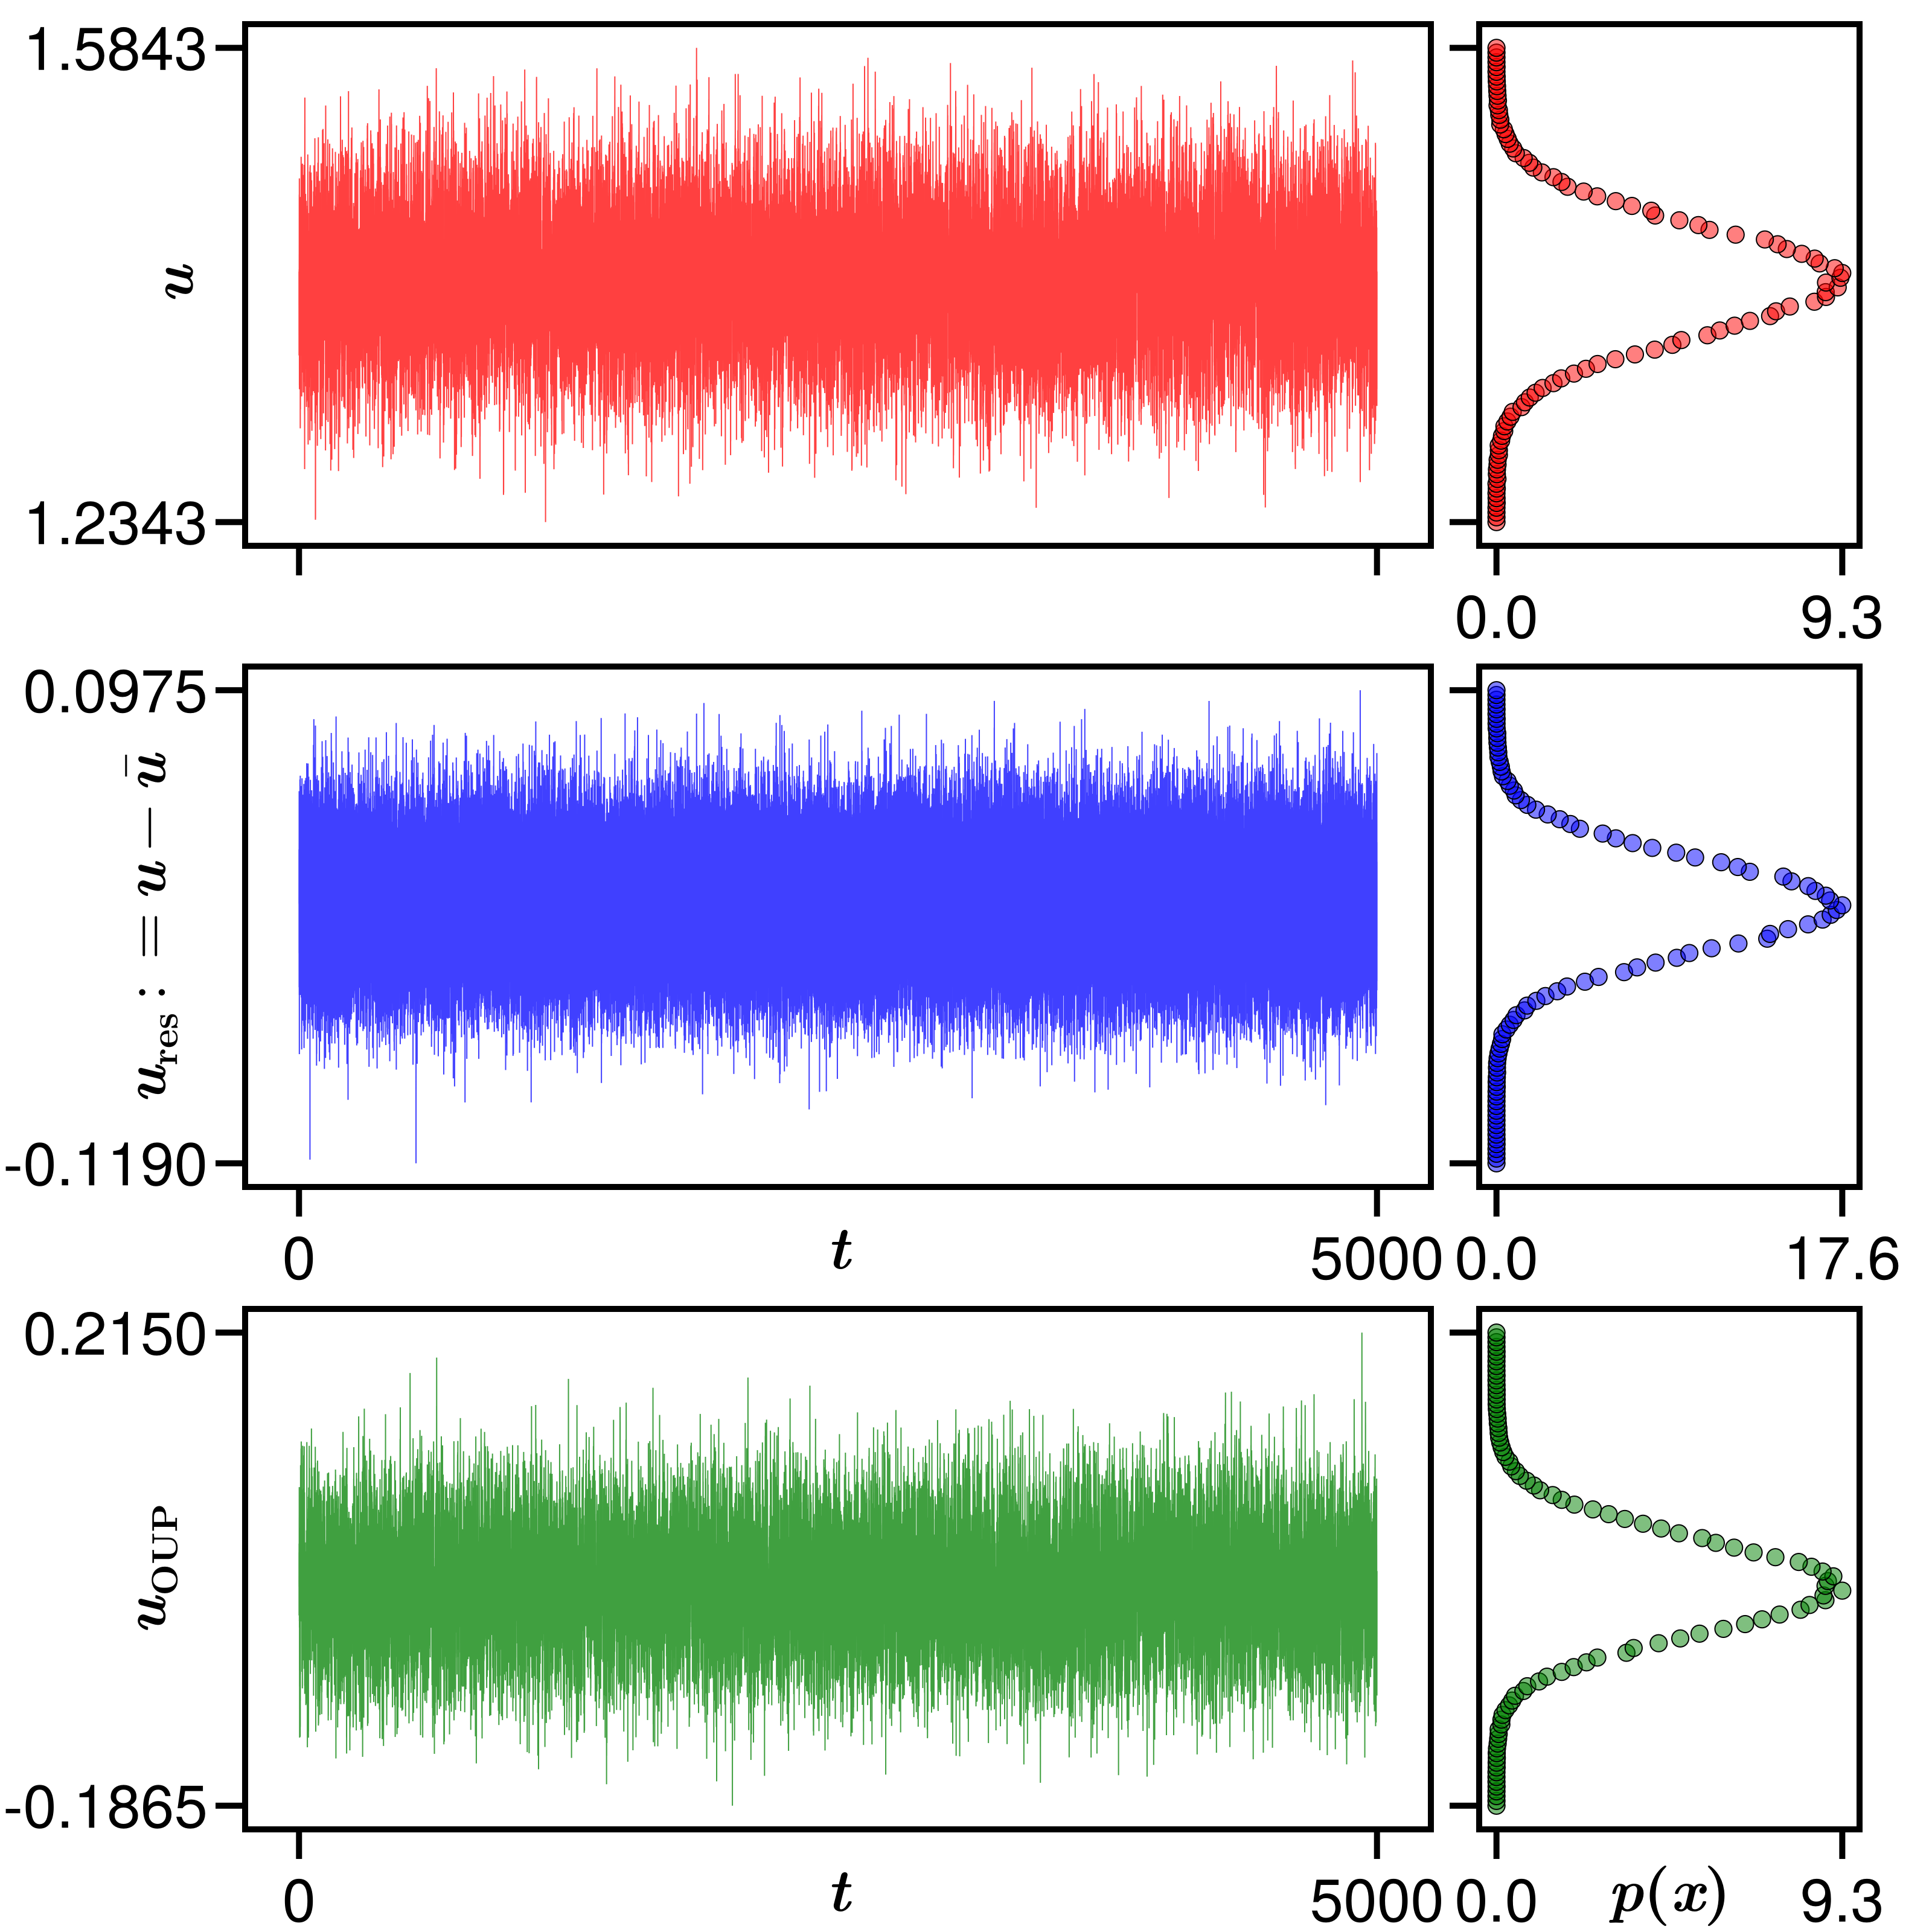
\includegraphics[keepaspectratio, width=\textwidth]{../figures/fig4.2.1.1.1.png}
    \caption{Timeseries and histograms of a saddle-node normal form (top, red) at fixed parameter value $\mu=-2$, its detrended residuals (middle, blue) and a topologically equivalent OUP (bottom, green) with $\theta\approx2.82$ and $x_{s}\approx1.414$. All $3$ systems have been simulated for $n=10^{5}$ realisations with (additive) noise level $\sigma=0.1$.}
    \label{fig4.2.1.1.1}
\end{figure}
The values $y_{n} =: p(x_{n})$ of this histogram can be put into \eqref{eq4.2.1.1.1}, which is now algebraic under the OUP assumption for the normalisation constant
\begin{equation}\label{eq2.4.1.1.2}
     V(x) = -D\ln\bigg(\sqrt{\frac{\theta}{\sigma^{2}\pi}}\;p(x)\bigg)\,,
\end{equation}
and the linear least-squares problem can thus be formulated
\begin{align}
     &\text{find}\;\,\{c_{0},c_{1},c_{2}\}\;\,\text{s.t.}\;\,\sqrt{\sum_{n=1}^{N_{\text{data}}}\big(U(x_{n}) - V_{n}\big)^{2}}\;\,\text{is minimal}\,, \label{eq4.2.1.1.3} \\ 
     &V(x_{n}) =: V_{n} = -D\ln\bigg(\sqrt{\frac{\theta}{\sigma^{2}\pi}}\;y_{n}\bigg)\,,\quad U(x)=\sum_{m=0}^{2}c_{m}x^{m}\,.\nonumber
\end{align}
\subparagraph{Generic cubic: topological equivalence with a saddle-node normal form}
For the purposes of EWS of incoming tipping-points we need to bound the basin of attraction of $x_{s}$ which necessarily entails the existence of at least $1$ unstable equilibrium $x_{u}$.
For that to be true we conclude that in order to derive the probabilistic EWS based on the escape problem from a potential well, the minimum working model is a (generic) cubic exponential
\begin{align*}
     U(x)            =& \sum_{m=0}^{3}c_{m}x^{m} = c_{0} + c_{1}x + c_{2}x^{2} + c_{3}x^{3}\,, \\
     \newprime{U}(x) =& \sum_{m=1}^{3}m\,c_{m}x^{m-1} = c_{1} + 2\,c_{2}x + 3\,c_{3}x^{2} \,, \\ 
     \pprime{U}(x) =& \sum_{m=2}^{3}m(m-1)c_{m}x^{m-2} = 2\,c_{2} + 6\,c_{3}x\,.
\end{align*}
As established in Example \ref{ex4.2.1.1} in order for the stationary FPE to exist in a cubic potential we need to truncate the domain at the unstable equilibrium $x_{u}$ and thereby impose reflecting BCs.
This already provides us with a constraint on the coefficients of the cubic potential since we want it to have a local minima (i.e. the stable equilibrium $x_{s}$) and a local maxima (i.e. the unstable equilibrium $x_{u}$).
This translates in imposing that $\newprime{U}(x)=0$, which is a quadratic polynomial, has to have exactly $2$ real and distinct roots $x_{1,2}$ which provides
\begin{equation}\label{eq4.2.1.1.4}
        x_{1,2}=\frac{-2c_{2}\pm\sqrt{\Delta}}{6c_{3}}\,,\;\Delta = 4(c_{2}^{2}-3c_{3}c_{1})>0\;\iff\;-\sqrt{3c_{3}c_{1}}>c_{2}>\sqrt{3c_{3}c_{1}}\,.
\end{equation}
Furthermore we can find closed-form expressions for both equilibria in terms of the unknown cubic coefficients since $\pprime{U}(x_{s})>0$ and $\pprime{U}(x_{u})<0$ leading us to
\begin{equation}\label{eq4.2.1.1.5}
        x_{s,u} = \pm \frac{1}{3c_{3}}\Big(\sqrt{c_{2}^{2}-3 c_{3}c_{1}}\mp c_{2}\Big)\,.
\end{equation}
Finally in order to choose the appropriate domain of integration we must be able to discern the case $x_{s}>x_{u}$, in which case the integration bounds are $[x_{u},+\infty)$, from $x_{s}<x_{u}$, which yields the integration domain $(-\infty,x_{u}]$ instead.
By using the closed-form expressions \eqref{eq4.2.1.1.5} we obtain
\begin{equation}\label{eq4.2.1.1.6}
        x_{s}>x_{u}\;\iff\;\frac{2}{3c_{3}}\Big(\sqrt{c_{2}^{2}-3c_{3}c_{1}}\Big)>0\;\iff\;c_{3}>0\,, 
\end{equation}
as expected.
We now use conditions \eqref{eq4.2.1.1.5}-\eqref{eq4.2.1.1.6} to write down the stationary solution of the FPE \eqref{eq4.2.1.2} explicitly 
\begin{equation}\label{eq4.2.1.1.7}
     p(x) = \Bigg(\int_{-\frac{1}{3c_{3}}\Big(\sqrt{c_{2}^{2}-3 c_{3}c_{1}}+c_{2}\Big)}^{+\infty}e^{-\frac{U(x)}{D}}dx\Bigg)^{-1}e^{-\frac{U(x)}{D}}\,.
\end{equation}
Notice that \eqref{eq4.2.1.1.7} is again trascendental given the fact that the improper integral does not have a closed-form expression for a generic cubic potential $U(x)=\sum_{m=0}^{3}c_{m}x^{m}$ and it has to be approximated either numerically by quadrature or other methods.
Now again we suppose that we have access to some timeseries data which we think of as the solution $x_{t}$ of a scalar, non-linear SDE with additive noise.
We want to quantify the probability of escape outside the basin of attraction of the stable equilibrium of the underlying SDE.
In order to do that we assume a cubic potential as a minimum model for our system.
Again we use the timeseries data to construct a histogram whose values $y_{n}$ correspond to an approximation of the stationary solution $p(x_{n})$ of the FPE \eqref{eq4.2.1.1.1}.
To quantify the coefficients $\{c_{m}\}_{m=0,\dots,3}$ we use \eqref{eq4.2.1.1.7}, together with condition \eqref{eq4.2.1.1.4}, to formulate the following contrained, non-linear optimisation problem
\begin{align}
     &\text{find}\;\,\{c_{0},c_{1},c_{2},c_{3}\}\;\,\text{s.t.}\;\,\sqrt{\sum_{n=1}^{N_{\text{data}}}\big(p(x_{n}) - y_{n}\big)^{2}}\;\,\text{is minimal}\,, \label{eq4.2.1.1.8} \\ 
     &p(x_{n}) =: p_{n} = \Bigg(\int_{-\frac{1}{3c_{3}}\Big(\sqrt{c_{2}^{2}-3 c_{3}c_{1}}+c_{2}\Big)}^{+\infty}e^{-\frac{U(x)}{D}}dx\Bigg)^{-1}e^{-\frac{U(x)}{D}}\,,\quad -\sqrt{3c_{3}c_{1}}>c_{2}>\sqrt{3c_{3}c_{1}}\,.\nonumber
\end{align}
\printbibliography
\end{document}
